% coding:utf-8

%----------------------------------------
%FOSAPHY, a LaTeX-Code for a summary of modern control theory
%Copyright (C) 2015, Mario Felder & Michi Fallegger

%This program is free software; you can redistribute it and/or
%modify it under the terms of the GNU General Public License
%as published by the Free Software Foundation; either version 2
%of the License, or (at your option) any later version.

%This program is distributed in the hope that it will be useful,
%but WITHOUT ANY WARRANTY; without even the implied warranty of
%MERCHANTABILITY or FITNESS FOR A PARTICULAR PURPOSE.  See the
%GNU General Public License for more details.
%----------------------------------------

\chapter{Digitale Regelung}

\section{Schematische Darstellung}
\begin{center}
	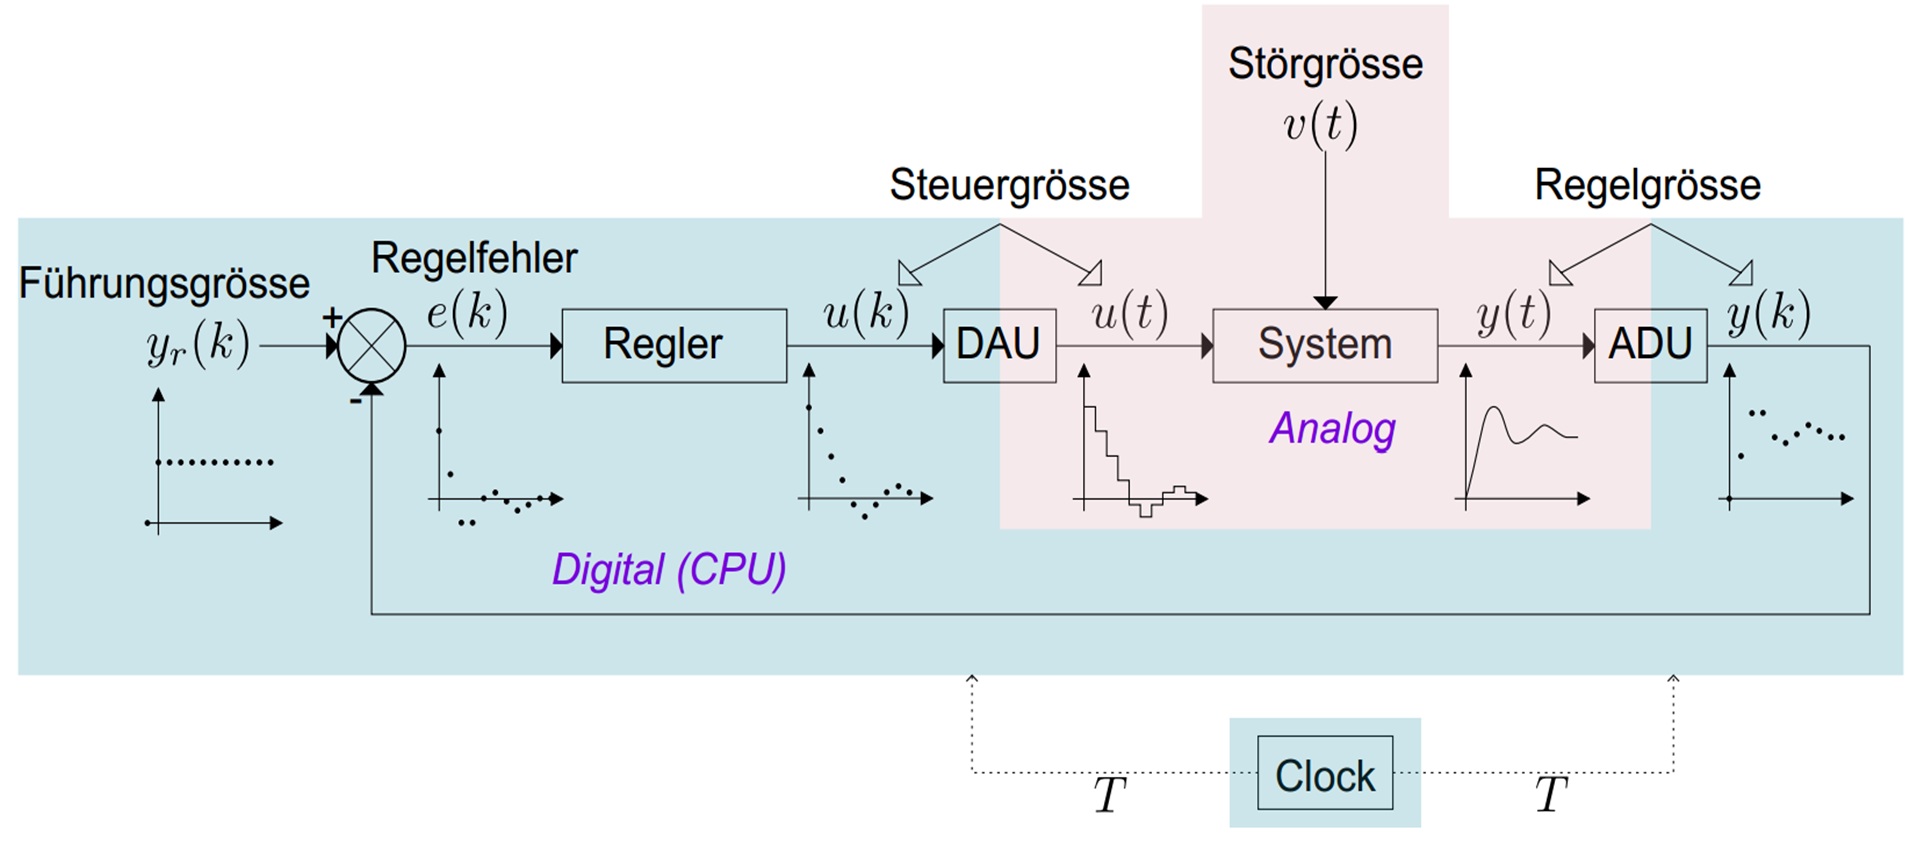
\includegraphics[scale = 0.3]{images/schematische_darstellung.png}
\end{center}
\[
	G(s)=\frac{Y(s)}{U(s)}\\ \rightarrow \\ H(z)=\frac{Y(z)}{U(z)} \\ \\
\]

\section{Wahl der Taktzeit}
Perfekte theoretische Rekunstruierung (unmöglich):
\[
	y(t) = \sum_{k=-\infty}^{\infty} y(kh) \frac{\sin\frac{\omega_e(t-kh)}{2}}{\frac{\omega_e(t-kh)}{2}}
\]
Wahl in der Praxis:
\[
	\omega_e > [10-20]\cdot \omega_{max}
\]

\section{Anti-Aliasing Filter}
\[\begin{aligned}
	G_{b,1} &= \frac{1}{\frac{1}{\omega_b}s+1}\\
	G_{b,2} &= \frac{1}{\frac{1}{{\omega_b}^2}s^2+\frac{\sqrt{2}}{\omega_b}s+1}\\
	G_{b,3} &= \frac{1}{\frac{1}{{\omega_b}^4}s^4+\frac{2.6131}{{\omega_b}^3}s^3+\frac{3.4142}{{\omega_b}^2}s^2+\frac{2.6131}{\omega_b}s+1}
\end{aligned}\]
\section{Direkter/Indirekter Regler}
\begin{center}
	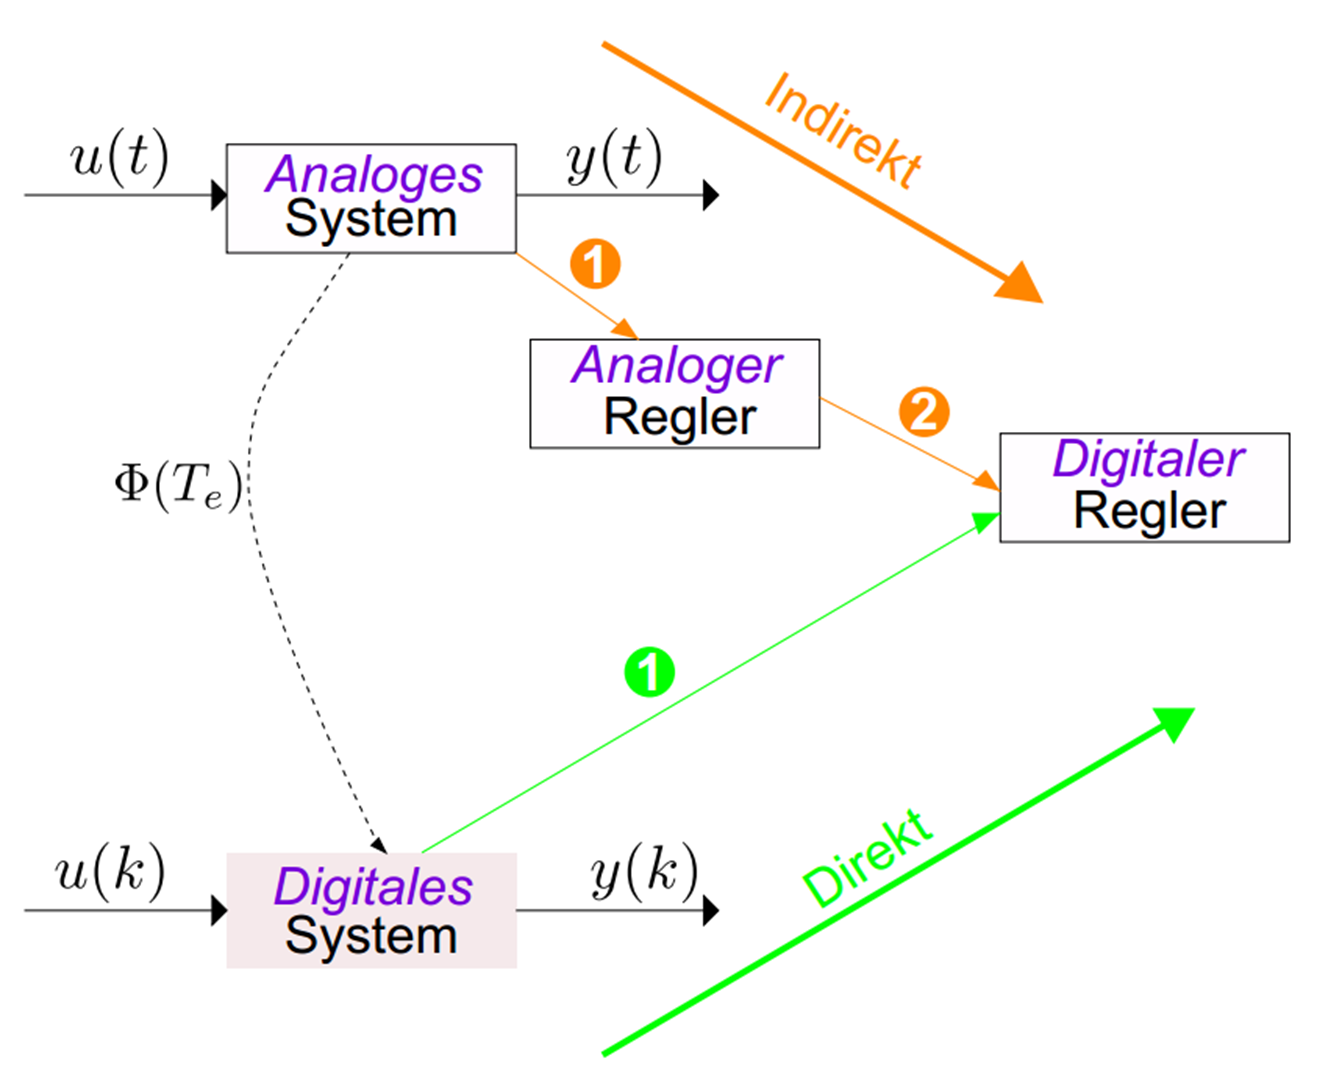
\includegraphics[scale = 0.25]{images/direkter_indirekter.png}
\end{center}

\section{Digitaler Regler}
\subsection{I Anteil}
Rückwärts-Rechteckregel
\[
	u_{i,d,r}(e[k])=u_{i,d,r}(e[k-1])+\frac{K_a}{T_{i,a}}e[k]\cdot T
\]
Trapezregel
\[
	u_{i,d,t}(e[k])=u_{i,d,t}(e[k-1])+\frac{K_a}{T_{i,a}}\cdot \frac{e[k]+e[k-1]}{2}\cdot T
\]
\subsection{D Anteil}
\[
	u_{d,d}(e[k])=K_aT_{d,a} \cdot \frac{e[k]-e[k-1]}{T}
\]
\subsection{Antireset-Windup}
\[\begin{aligned}
	u_{nosat}[k] &= u_p[k] + u_i[k-1] + u_d[k]	\\
	\textrm{if}\ u_{nosat}[k]&>u_{sat,max} \rightarrow {u[k] =  u_{sat,max} } \\
	\textrm{else if}\ u_{nosat}[k]&<u_{sat,min} \rightarrow u[k] =  u_{sat,min} \\
	u_i[k]&= u_i[k-1]+K_a\frac{T}{Ti}\cdot\frac{e[k]+e[k-1]}{2}+\frac{T}{T_r}(u[k]-u[k]_{nosat})
\end{aligned}\]
Ohne ARW:
\[\begin{aligned}
	u_i[k]&= u_i[k-1]+K_a\frac{T}{Ti}\cdot\frac{e[k]+e[k-1]}{2} \\
	u_{nosat}[k] &= u_p[k] + u_i[k] + u_d[k]	\\
	\textrm{if}\ u_{nosat}[k]&>u_{sat,max} \rightarrow {u[k] =  u_{sat,max} } \\
	\textrm{else if}\ u_{nosat}[k]&<u_{sat,min} \rightarrow u[k] =  u_{sat,min} \\
\end{aligned}\]

\section{z-Transformation}
\begin{center}
	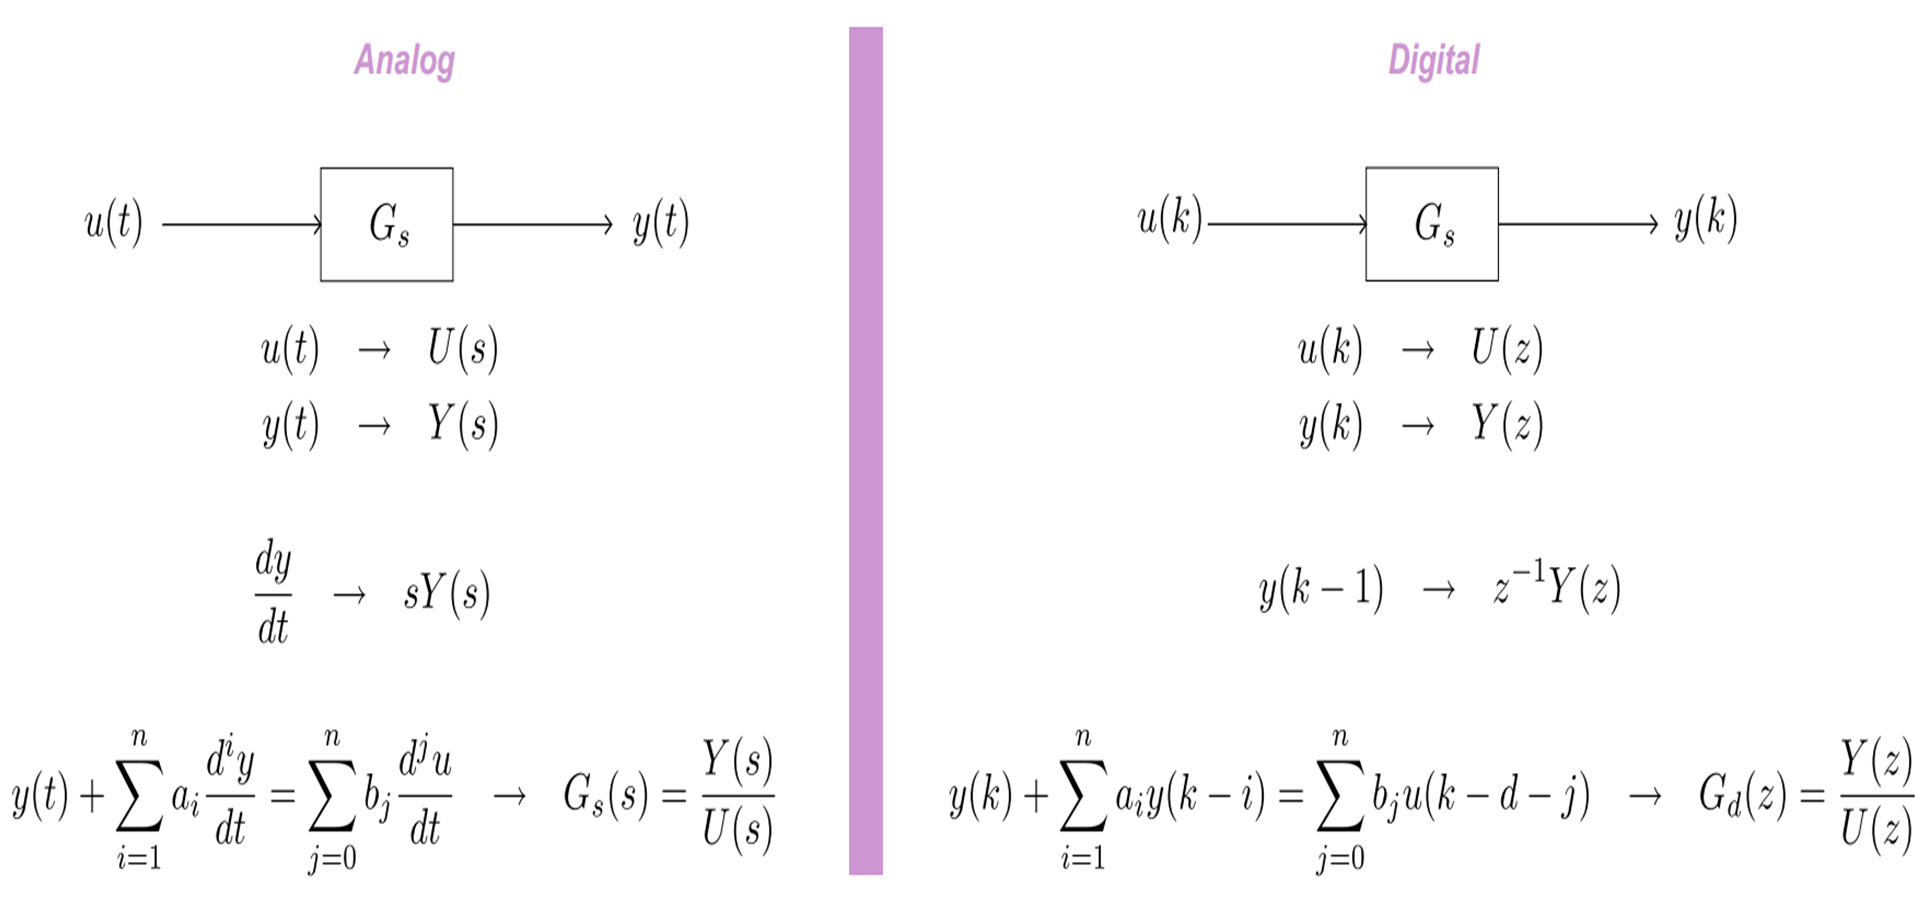
\includegraphics[scale = 0.25]{images/z_transf.png}
\end{center}
\subsection{Definition}
\[
	W(z) = Z\{w[k]\} = \sum_{k=0}^{\infty}w[k]z^{-k}
\]
\subsection{Signale}
Impuls:
\[
	Z\left\lbrace I_i[k]\right\rbrace  =z^{-l} \qquad \begin{cases}\textrm{1 if k $=$ l}\\\textrm{0 if k $\neq$ l}\end{cases}
\]
Sprungantwort:
\[
	Z\left\lbrace S_i[k]\right\rbrace  =\sum_{i=l}^{\infty}z^{-i}=z^{-l}\frac{z}{z-1} \qquad \begin{cases}\textrm{1 if k $\geq$ l}\\\textrm{0 if k $<$ l}\end{cases}
\]

\subsection{Eigenschaften der z-Transformation}
Linearität 1:
\[
	Z(\{w_1[k]\}+\{w_2[k]\}) = Z\{w_1[k]\} + Z\{w_2[k]\}
\]
Linearität 2:
\[
	Z(a\{w_1[k]\}) = a \cdot Z\{w_1[k]\}
\]
Zeitverschiebung:
\[
	Z(\{w_1[k-d]\}) = z^{-d}W(z)
\]
Initialwert:
\[
	w[0] = \lim\limits_{z\rightarrow\infty}W(z)
\]
Finalwert:
\[
	w[\infty] = \lim\limits_{z\rightarrow 0}(z-1)W(z)
\]

\section{z-Übertragungsfunktion}
Impulsantwort beschreibt das System:
\[
	y[k] = \sum_{l=0}^{k}u[l] \cdot g[k-l]
\]

\subsection{Übertragung der Regelstrecke}
\begin{center}
	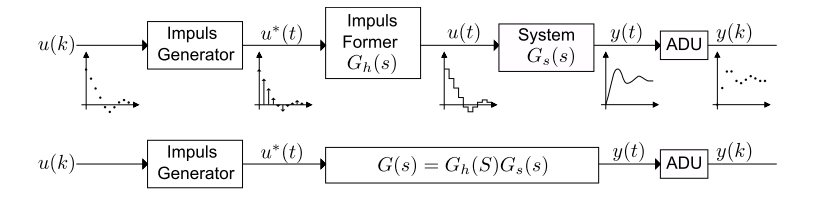
\includegraphics[width=.8\textwidth]{./images/regelstrecke}
\end{center}

\[\begin{aligned}
	H(z) &= Z\{L^{-1}\{G_h(s)G_s(s)\}|_{t=kT}\} \\
		&= (1-z^{-1})Z\left\lbrace L^{-1}\left.\left\lbrace\frac{G_s(s)}{s}\right\rbrace\right| _{t=kT}\right\rbrace
\end{aligned}\]

\section{Laplace- $\rightarrow$ z-Übertragungsfunktion}
\[
	G(s) = \frac{U(s)}{E(s)} = K \left( 1 + \frac{1}{T_is}+T_ds\right) \ \rightarrow \ G(z) =  \frac{U(z)}{E(z)} = ?
\]

\subsection{Transformation}
Rückwärts-Rechteckregel:
\[
	\dot{e}[kT] = \frac{e[kT]-e[kT-T]}{T} \qquad \rightarrow \qquad s = \frac{z-1}{Tz}
\]
Vorwärts-Rechteckregel:
\[
	\dot{e}[kT] = \frac{e[kT+T]-e[kT]}{T} \qquad \rightarrow \qquad  s = \frac{z-1}{T}
\]
Trapezregel:
\[
	\int_{0}^{t}e[\tau]\di\tau = \sum_{i=0}^{\frac{k}{t}=kT}\frac{e[i]+e[i-1]}{2} \qquad \rightarrow \qquad s = \frac{2}{T} \frac{z-1}{z+1}
\]

\section{Stabilität}
\begin{center}
	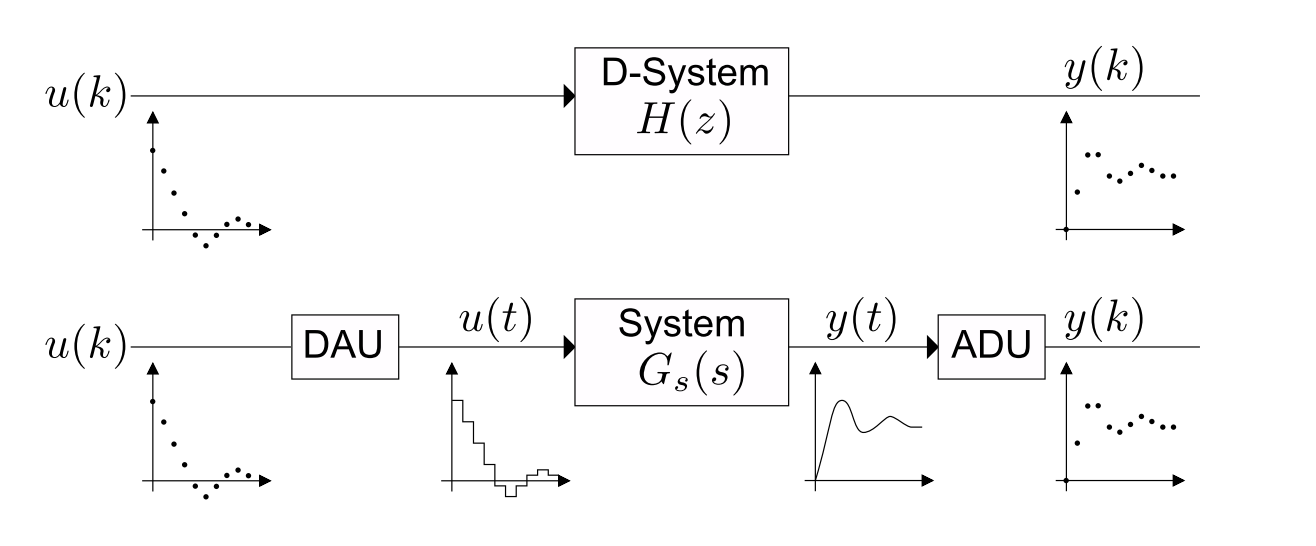
\includegraphics[width=.8\textwidth]{./images/stabilitat}
\end{center}
Ein digitales LZI-Glied ist stabil, wenn die Pole seiner z-Übertragungsfunktion $H(z)$ im Einheitskreis liegen.

\subsection{Analyse mit der Impulsantwort}
Das System ist stabil wenn
\[ \sum_{k=0}^{\infty}|g[k]|<\infty \]

\section{Zusammenhang Pole Laplace $\leftrightarrow$ z}
\[\begin{aligned}
	\frac{c}{s-s_1} \qquad &\rightarrow \qquad \frac{cz}{z-\e^{s_1^T}} \\
	s_1 = \sigma_1 + \im\omega_1 \qquad &\rightarrow \qquad  z_1=\e^{s_1T} = \e^{\sigma_1T}\e^{\im\omega_1T}
\end{aligned}\]

\[
	|z| = \e^\sigma \qquad \arg(z) = \omega T
\]

\subsection{Periodizität}
\[
	\omega_e = \frac{2\pi}{T}
\]

\[
	z = \e^{(s+\im\omega_e)T} = \e^{sT}
\]

\begin{figure}[th]
	\begin{subfigure}[b]{0.45\textwidth}
		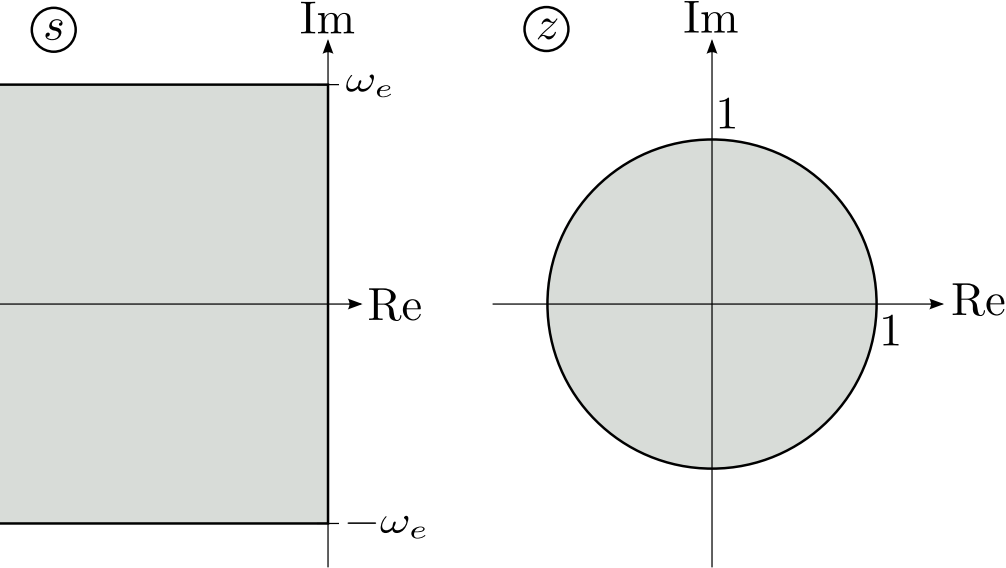
\includegraphics[width=\textwidth]{./images/mapping1}
		\caption{Mapping 1}
	\end{subfigure}
	\hfill
	\begin{subfigure}[b]{0.45\textwidth}
		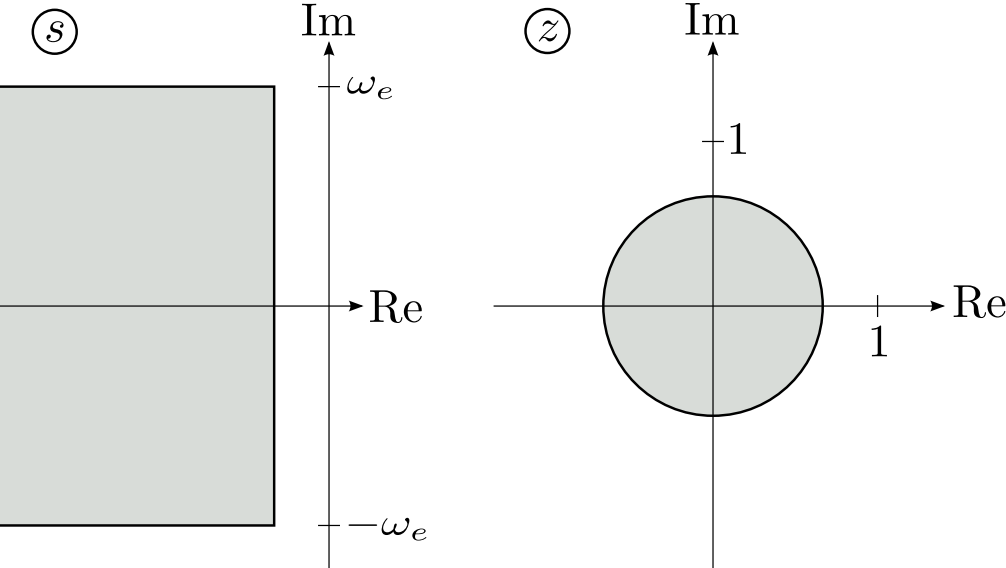
\includegraphics[width=\textwidth]{./images/mapping2}
		\caption{Mapping 2}
	\end{subfigure}
	\\\\
	\begin{subfigure}[b]{0.45\textwidth}
		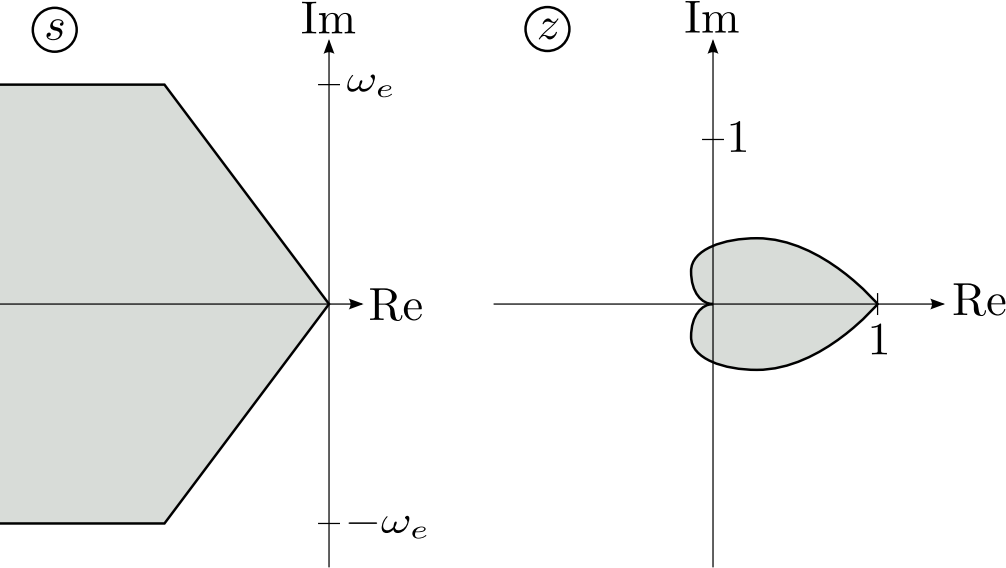
\includegraphics[width=\textwidth]{./images/mapping3}
		\caption{Mapping 3}
	\end{subfigure}
	\hfill
	\begin{subfigure}[b]{0.45\textwidth}
		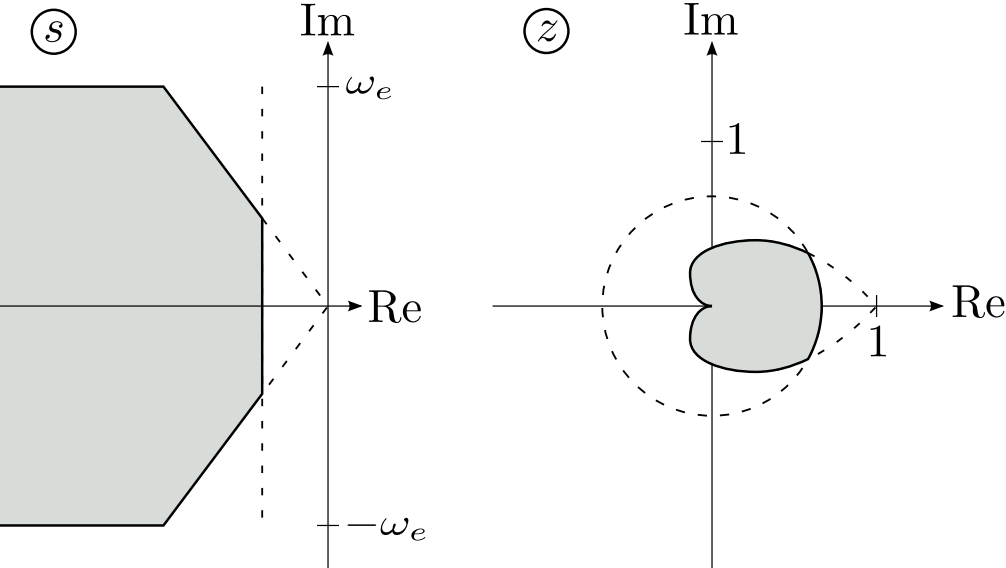
\includegraphics[width=\textwidth]{./images/mapping4}
		\caption{Mapping 4}
	\end{subfigure}
\end{figure}

\section{Wichtige Übertragungsfunktionen}
\subsection{z-Übertragung des offenen Regelkreises}
\[
	\frac{Y(z)}{E(z)} = K(z)H(z)
\]
\begin{center}
	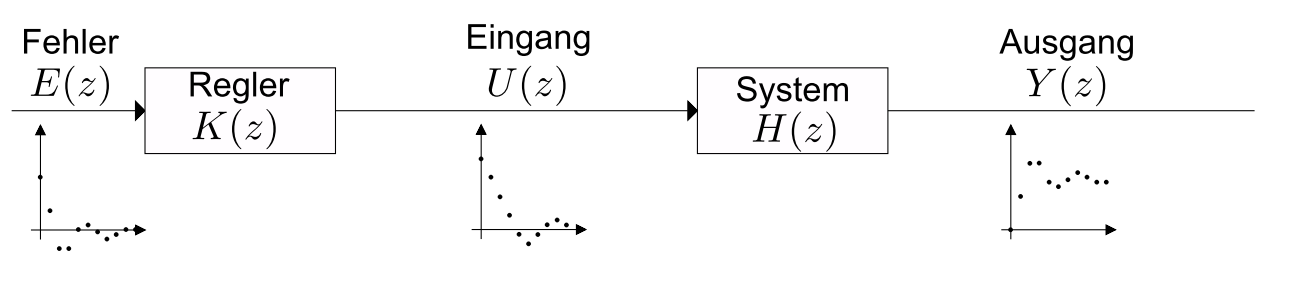
\includegraphics[width=.8\textwidth]{./images/rol}
\end{center}

\subsection{Führungsübertragungsfunktion}
\[
	\frac{Y(z)}{Y_r(z)} = \frac{K(z)H(z)}{1+K(z)H(z)}
\]
\begin{center}
	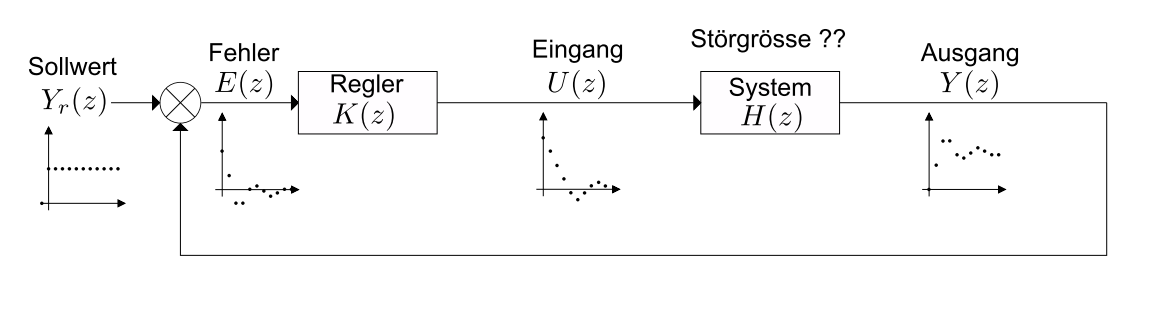
\includegraphics[width=.8\textwidth]{./images/rcl}
\end{center}

\subsection{Störübertragungsfunktion}
\[
	Y(z) = \frac{K(z)H(z)}{1+K(z)H(z)}Y_r(z)+\frac{Z\{L^{-1}\{G(s)V(s)\}\}}{1+K(z)H(z)}
\]
\begin{center}
	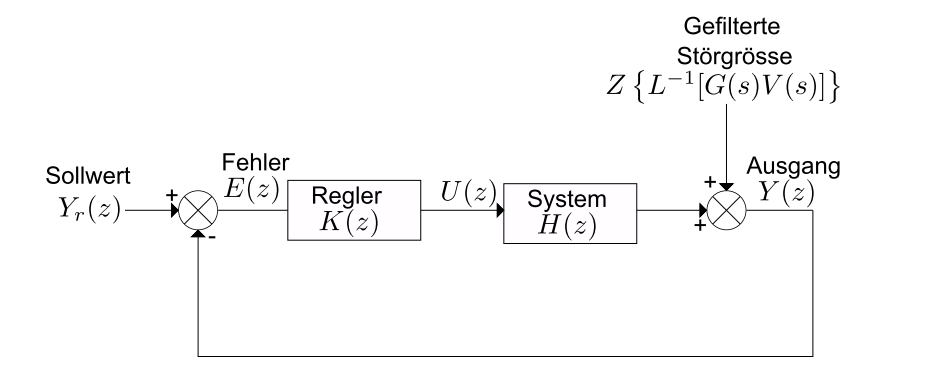
\includegraphics[width=.8\textwidth]{./images/storueb}
\end{center}

mit Störfunktion $v(t) = a$:
\[
	Y(z) = \frac{K(z)H(z)}{1+K(z)H(z)}Y_r(z)+\frac{H(z)}{1+K(z)H(z)}V(z) \qquad \textrm{mit } V(z) = \frac{az}{z-1}
\]

\section{Diskrete Zustandsraumdarstellung}
Analog:
\[\begin{aligned}
	\dot{x}(t) &= Ax(t) + Bu(t)\\
	y(t) &= Cx(t) + Du(t)
\end{aligned}\]
Digital:
\[\begin{aligned}
	x[k+1] &= A_dx[k] + B_du[k]\\
	y[k+1] &= C_dx[k] + D_du[k]
\end{aligned}\]
Transformation
\[\begin{aligned}
	A_d &= \e^{AT}\\
	B_d &= \int_{0}^{T}\e^{A\tau}\di\tau B\\
	C_d &= C\\
	D_d &= D
\end{aligned}\]

\section{Diskreter Frequenzgang}
\subsection{Eigenschaften}
Periodizität
\[
	H(\e^{\im(\omega+\frac{2k\pi}{T})T})=H(\e^{\im\omega T})
\]
Symmetrie für $A(\omega)$
\[
	A(-\omega) = A(\omega)
\]
Asymmetrie für $\varphi(\omega)$
\[
	\varphi(-\omega) = -\varphi(\omega)
\]

\subsection{Nyquist Frequenz}
Die Analyse des Frequenzganges beschränkt sich auf:
\[
	\omega \in [0,\omega_N] \qquad \omega_N = \frac{\pi}{T}
\]

\subsection{Bode-Diagramm}
\begin{enumerate}
	\item $H(z)$ herleiten
	\item $z$ durch $\e^{\im\omega T}$ ersetzten
	\item $|H(\e^{\im\omega T})| = \sqrt{Re\{\e^{\im\omega T}\}^2+Im\{H(\e^{\im\omega T})\}^2}$
	\item $\arg H(\e^{\im\omega T}) = \arctan \left(\frac{Im\{H(\e^{\im\omega T})\}}{Re\{H(\e^{\im\omega T})\}}\right)$
\end{enumerate}